\subsection{Architettura di dettaglio: Strategy pattern} 
\begin{figure}[hb]
	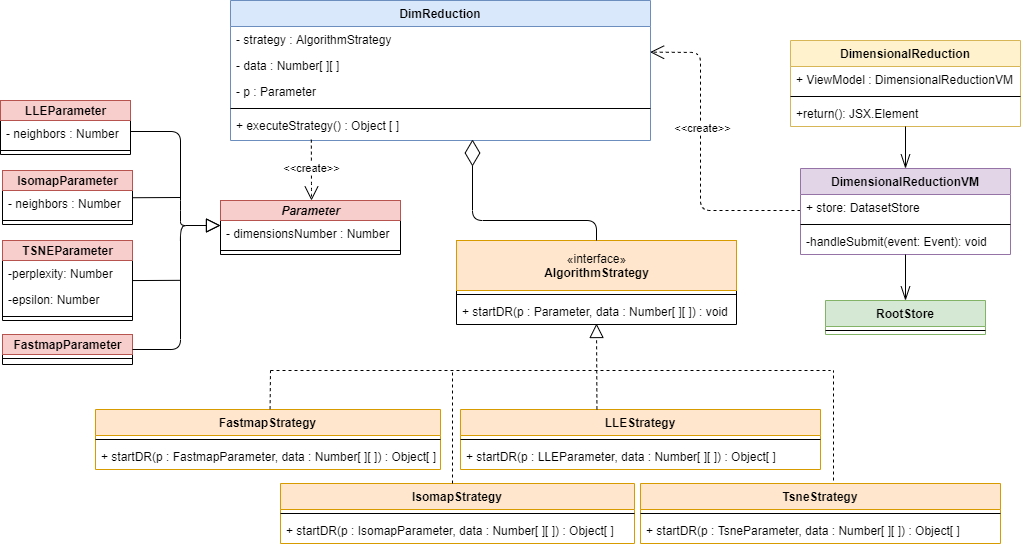
\includegraphics[width=17cm]{Images/StrategyPattern}
	\centering
	\caption{Strategy pattern per la scelta dell'algoritmo di riduzione dimensionale}
\end{figure}
Nella figura sopra è mostrata la funzionalità di riduzione dimensionale sui dati caricati dall'utente.
Per l'implementazione dei vari algoritmi viene utilizzato lo strategy pattern. In particolare:
\begin{itemize}
	\item \textbf{DimensionalReduction} è il componente React che si occupa solo di ritornare gli elementi HTML che compongono questa parte di vista;
	\item \textbf{DimensionalReductionVM} è il rispettivo view-model che ne contiene tutta la logica. Questo prende i dati dal RootStore (nello specifico dal \textit{DatasetStore}) e crea il contesto DimReduction;
	\item \textbf{DimReduction} si occupa di creare i parametri con i valori impostati dall'utente dalla vista. A seconda del valore del suo attributo \texttt{strategy} crea la corretta classe di parametri e chiama attraverso \texttt{executeStrategy()} il metodo \texttt{startDR()} sull'algoritmo scelto;
	\item \textbf{AlgorithmStrategy} è l'interfaccia implementata dalle famiglia di classi concrete degli algoritmi, facilitandone l'estensibilità.
\end{itemize} 

Infine \texttt{startDR()} esegue la riduzione dimensionale sui dati utilizzando i metodi forniti dalla libreria Druid.js e ritorna le nuove dimensioni.
